\documentclass[11pt,a4paper,spanish]{book}  % book, article

\usepackage[english]{babel}
\usepackage[utf8]{inputenc}
% Paquetes para incluir graficos:
\usepackage{graphics}
\usepackage{graphicx}
\usepackage{epstopdf}
% Tratamiento de graficos
\usepackage{picture}
% Colores
\usepackage[usenames]{color}
% Texto preformateado
\usepackage{verbatim}
\usepackage{listings}
% Hipervinculos (indice y URLs)
\usepackage{hyperref}
% Matematicas
\usepackage{amsfonts}
\usepackage{amsmath}
\usepackage{amsthm}
\usepackage{amssymb}
\usepackage{anysize}
\usepackage{caption}
\usepackage{geometry}
\usepackage[final]{pdfpages}
\usepackage{cite}
\usepackage{natbib}
\usepackage[numbib,notlof,notlot,nottoc]{tocbibind}

\newcommand{\HRule}{\rule{\linewidth}{0.5mm}}

%%PER EL CODI EN C%%%
\usepackage{listings}
\lstset{ %
language=C++,                % choose the language of the code
basicstyle=\footnotesize,       % the size of the fonts that are used for the code
numbers=left,                   % where to put the line-numbers
numberstyle=\footnotesize,      % the size of the fonts that are used for the line-numbers
stepnumber=1,                   % the step between two line-numbers. If it is 1 each line will be numbered
numbersep=5pt,                  % how far the line-numbers are from the code
backgroundcolor=\color{white},  % choose the background color. You must add \usepackage{color}
showspaces=false,               % show spaces adding particular underscores
showstringspaces=false,         % underline spaces within strings
showtabs=false,                 % show tabs within strings adding particular underscores
frame=single,           % adds a frame around the code
tabsize=2,          % sets default tabsize to 2 spaces
captionpos=b,           % sets the caption-position to bottom
breaklines=true,        % sets automatic line breaking
breakatwhitespace=false,    % sets if automatic breaks should only happen at whitespace
escapeinside={\%*}{*)}          % if you want to add a comment within your code
}

%%%%%%%% Entornos teorema, definiciÛn, comentario, ... %%%%%%%%
\swapnumbers  % Poner el numero del teorema ANTES del teorema.

\theoremstyle{definition}  % Titulo en negrita y texto plano

\newtheorem{definicion}{Definicion}[chapter]
\newtheorem{ejemplo}[definicion]{Ejemplo}
\newtheorem{comentario}[definicion]{Comentario}
\newtheorem{propiedades}[definicion]{Propiedades}
\newtheorem*{objetivo}{Objetivo}
\newtheorem*{idea}{Idea}

\theoremstyle{plain}  % Titulo en negrita y texto en cursiva.
\newtheorem{teorema}[definicion]{Teorema}
\newtheorem{proposicion}[definicion]{ProposiciÛn}
\newtheorem{corolario}[definicion]{Corolario}
\newtheorem{lema}[definicion]{Lema}

\theoremstyle{remark}  % Titulo en cursiva y texto plano
\newtheorem*{observacion}{ObservaciÛn}
\newtheorem*{ejercicio}{Ejercicio propuesto}
\newtheorem*{pregunta}{Pregunta}

%%%%%%%% Formato cÛdigo incluido %%%%%%%% 
\lstset{ %
%language=Octave,                % choose the language of the code
basicstyle=\footnotesize,       % the size of the fonts that are used for the code
numbers=left,                   % where to put the line-numbers
numberstyle=\footnotesize,      % the size of the fonts that are used for the line-numbers
stepnumber=1,                   % the step between two line-numbers. If it's 1 each line 
                                % will be numbered
numbersep=5pt,                  % how far the line-numbers are from the code
%backgroundcolor=\color[rgb]{0.8,0.8,0.8},  % choose the background color. You must add \usepackage{color}
showspaces=false,               % show spaces adding particular underscores
showstringspaces=false,         % underline spaces within strings
showtabs=false,                 % show tabs within strings adding particular underscores
frame=single,	                % adds a frame around the code
tabsize=2,	                % sets default tabsize to 2 spaces
captionpos=b,                   % sets the caption-position to bottom
breaklines=true,                % sets automatic line breaking
breakatwhitespace=false,        % sets if automatic breaks should only happen at whitespace
title=\lstname,                 % show the filename of files included with \lstinputlisting;
                                % also try caption instead of title
escapeinside={\%*}{*)},         % if you want to add a comment within your code
morekeywords={*,...}            % if you want to add more keywords to the set
}




%\marginsize{3 cm}{2 cm}{2 cm}{2.5 cm}

%\title{\textbf{Project Handbook for Development Projects}}
%\author{Carolina Millet \\ Xavier Bush}
%\date{October 2014}		% Comentar para que aparezca la fecha de hoy
\newgeometry{
    top=35mm,
    bottom=30mm,
    outer=30mm,
    inner=30mm,
}

\begin{document}


\begin{titlepage}
\begin{center}


\textsc{\LARGE Kungliga Tekniska Högskolan}\\[1.5cm]

\textsc{\Large ~}\\[-0.5cm]


{ \huge \bfseries \textbf{Project Report} \\

\HRule

 Noise and echo cancellation in a teleconference\\[0.4cm]}

\HRule \\[1.1cm]

		\begin{figure}[h]
		\centering
		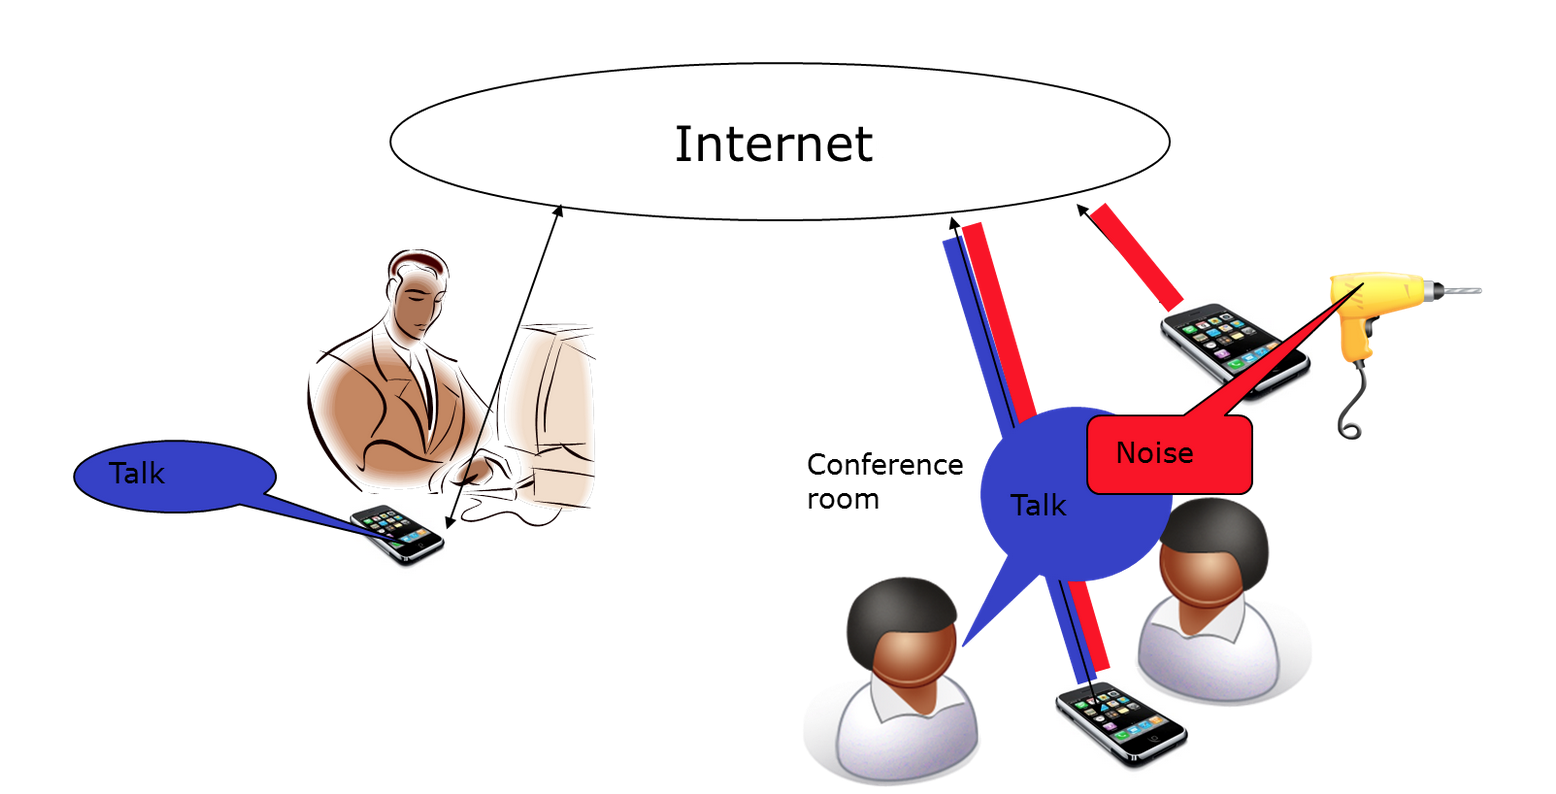
\includegraphics[width=10cm]{images/other/scenario}
		\label{scenario}
		\end{figure}

% Author and supervisor
\begin{minipage}{0.4\textwidth}
\begin{flushleft}
\emph{Authors:}\\
Animesh DAS \\ Jonas SEDIN \\ Mohammad ABDULLA \\ Thomas GAUDY \\ Xavier BUSH
\end{flushleft}
\end{minipage}
~
\begin{minipage}{0.4\textwidth}
\begin{flushright}
\emph{Advisor:}\\
Per ZETTERBERG
\end{flushright}
\end{minipage}

\vfill

% Bottom of the page
{\large Spring 2015} \\[1cm]
\end{center}



\end{titlepage}
\restoregeometry



\pagebreak\tableofcontents
\pagebreak

\chapter{Background}

	\section{Introduction of the problem}
	
	Nowadays the scenarios with phone calls involved are increasing every day. This fact implies an increase of the probability of being in a noisy scenario, specially in big cities. As a result of the discomfort that the users suffer and claim, engineering and science have worked with different approaches to solve this problem.
	
	The nature and origin of the noise affects directly to the solutions to implement, being it one of the biggest obstacles: a high performance of the implementation in different situations is a technical and a comfort requierement. Considering that the noise can be white or colored, coming from a concrete source or considered as background noise, and it could last from miliseconds to minutes, the solutions have to be adaptive enough to follow the noise and cancel it in the best possible way. 
	
	

	\section{Historical Overview}
	
	\section{Goal}
	
	\section{Organization}


\chapter{Methodology}

\chapter{Theory}

\chapter{Android}

\chapter{Conclusions}

%\include{Chapter1}			% Incluye "Chapter1.tex"


%%%%%%%% Fin del documento %%%%%%%% 
\end{document}